\section{Introdução}

Neste trabalho estudaremos resultados que tratam da tarefa de representar um conjunto de funções por meio de outro, podendo essa representação ser exata ou aproximada.
Esse é um tema amplo, presente em diversas áreas da matemática, tanto pura quanto aplicada.
Faremos esse estudo em alguns contextos diferentes, sendo o principal deles o da aproximação de funções contínuas por meio de redes neurais.

Começaremos pelo teorema da aproximação de Weierstrass, que estabelece a viabilidade de aproximar arbitrariamente bem funções contínuas em um intervalo da reta por meio de polinômios.
Inicialmente provado por Weierstrass em 1885, novas demonstrações surgiram com o tempo.
A que apresentaremos --- retirada de \cite{weierstrass} --- ainda fornecerá uma forma de, dada uma função contínua, obter os polinômios que a aproximam.
Essa é uma peculiaridade desse teorema, pois as provas seguintes não são construtivas.

Escolhemos iniciar com esse resultado por sua demonstração ser elementar, não exigindo mais que um curso de análise na reta.
Além disso, ele trata de aproximações em um contexto mais simples, com apenas uma variável e no qual as funções aproximadoras, os polinômios, são lineares com relação aos seus coeficientes, os parâmetros da aproximação.
Com isso, esperamos acostumar o leitor ao tipo de questão que nos é de interesse.

Em seguida, moveremos nossa atenção para um dos problemas apresentados por David Hilbert no Congresso Internacional de Matemáticos de 1900, mais especificamente, o \( 13^{ \circ } \).
Hilbert postulou (utilizando a linguagem matemática de sua época) que existem funções contínuas de \( \I^{ 3 } \) em \( \R \), onde \( \I = [0, 1] \), que não podem ser expressas por meio da composição e adição de funções de \( \R^{ 2 } \) em \( \R \).
Décadas após ser postulada, essa conjectura eventualmente foi demonstrada \emph{falsa}.
A prova foi dada por Vladimir Igorevich Arnol'd, 14 anos após a morte de Hilbert.
Ele e seu orientador de Doutorado, Andrej Nikolajewitsch Kolmogorov, provaram que, na verdade, toda função contínua \( f : \I^{ n } \to \R \) pode ser expressa como composições e adições de funções contínuas de \( \R \to \R \).
A formulação exata que apresentaremos --- obtida de \cite{hilbert} --- é ainda mais forte que essa.

Naturalmente, a diferença mais óbvia desse resultado para o anterior é que agora nós temos representações \emph{exatas} para nossas funções de interesse, não apenas aproximações.
Além disso, esse é um contexto que envolve múltiplas variáveis e no qual as funções aproximadoras não são lineares em seus parâmetros.
Portanto, é de se esperar que a demonstração apresentada seja mais complexa.
De fato, apesar de não ser extremamente complicada, ela envolve conceitos e resultados sobre espaços métricos aos quais julgamos apropriado dedicar um apêndice.

O último e principal resultado sobre aproximações que apresentaremos é o teorema da aproximação universal, como formulado em \cite{cybenko89}:
\begin{TAU}
    Seja \( \sigma : \R \to \R \) uma função contínua discriminatória qualquer.
    Então, dada qualquer \( f : \I^{ n } \to \R \), contínua, e \( \varepsilon > 0 \), existe uma soma, \( G : \I^{ n } \to \R \), da seguinte forma:
    \begin{equation}
        G(x) = \sum_{ j=1 }^{ N } \alpha_{ j } \sigma(y_{ j }^{ T }x + \theta_{ j })
        \label{eq: neural_func_form}
    ,\end{equation}
    onde \( \alpha_{ j }, \theta_{ j } \in \R \) e \( y_{ j } \in \R^{ n } \), tal que \[
        \abs{ G(x) - f(x) } < \varepsilon
    \]
    para todo \( x \in \I^{ n } \).
\end{TAU}

Aqui \( y_{ j }^{ T } \) é o transposto do vetor \( y_{ j } \), de modo que \( y_{ j }^{ T }x \) é o produto interno usual de \( \R^{ n } \).
A definição de função discriminatória será dada posteriormente.

Antes de apresentar comentários sobre esse teorema, é prudente explicar sua relação com redes neurais.
Como descrito em \cite{lipmann}, as redes neurais artificiais são algoritmos de computação que surgiram como uma tentativa de espelhar o funcionamento de redes neurais orgânicas, como o cérebro humano.
Em essência, seu objetivo é ``atingir bom desempenho por meio da densa interconexão de elementos computacionais simples.''

Na prática, existem várias formas de atingir esse objetivo.
No tipo de rede ao qual daremos enfoque, o processo de computação é realizado por um conjuntos de nós, organizados em camadas ordenadas, em que a camada inicial é composta por \( n \) nós de \verb|input| e a camada final, por \( m \) nós de \verb|output|.
Entre eles a rede pode possuir camadas intermediárias de tamanho variado.
Dados \( n \) valores reais para os nós de \verb|input|, a rede produz, nos nós de \verb|output|, \( m \) valores, também reais.
Logo, ela pode ser considerada uma função de \( \R^{ n } \) em \( \R^{ m } \).

\begin{figure}[h]
    \begin{center}
        % !TeX root = ../main.tex

\tikzset{%
  every neuron/.style={
    circle,
    draw,
    minimum size=1cm
  },
  neuron missing/.style={
    draw=none, 
    scale=3,
    text height=0.3cm,
    execute at begin node=\color{black}$\vdots$
  },
}

\vspace{.6cm}

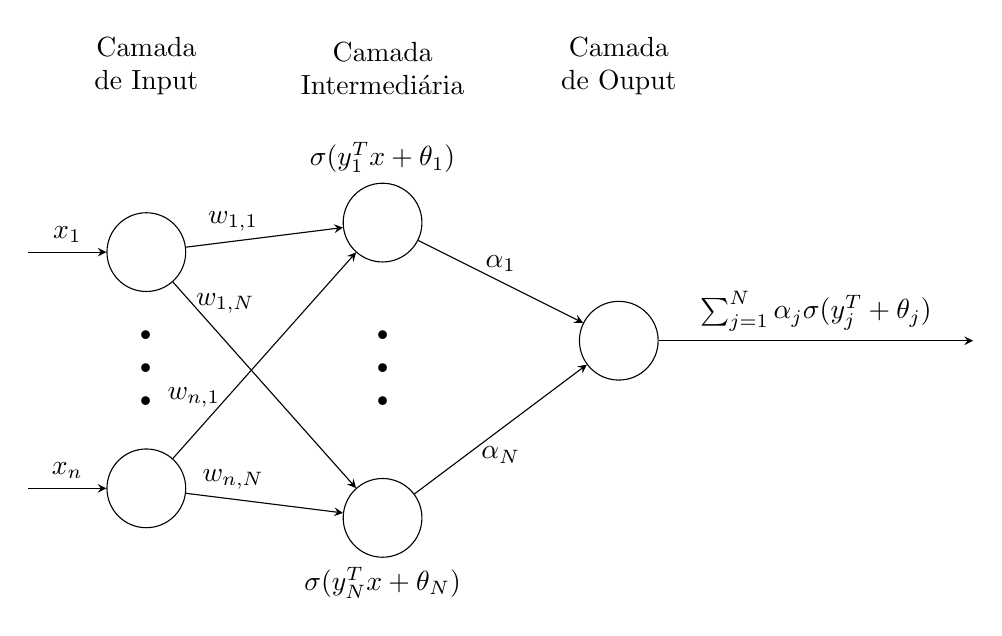
\begin{tikzpicture}[x=1.5cm, y=1.5cm, yshift=-1, >=stealth]

\foreach \m/\l [count=\y] in {1,missing,2}
  \node [every neuron/.try, neuron \m/.try] (input-\m) at (0,1.75-\y) {};

\foreach \m [count=\y] in {1,missing,2}
  \node [every neuron/.try, neuron \m/.try ] (hidden-\m) at (2,2.25-\y*1.25) {};

\foreach \m [count=\y] in {1}
  \node [every neuron/.try, neuron \m/.try ] (output-\m) at (4,1-\y) {};

\foreach \l [count=\i] in {1,n}
  \draw [<-] (input-\i) -- ++(-1,0)
    node [above, midway] {$x_\l$};

%% \foreach \l [count=\i] in {1,n}
%%   \node [above] at (hidden-\i.north) {$H_\l$};
\node [above] at (hidden-1.north) {\( \sigma (y_{ 1 }^{ T }x + \theta_{ 1 }) \)};
\node [below] at (hidden-2.south) {\( \sigma (y_{ N }^{ T }x + \theta_{ N }) \)};

\foreach \l [count=\i] in {1}
  \draw [->] (output-\i) -- ++(3,0)
    node [above, midway] {\( \sum_{ j=1 }^{ N } \alpha_{ j } \sigma (y_{ j }^{ T } + \theta_{ j }) \)};

%% \foreach \i in {1,...,2}
%%   \foreach \j in {1,...,2}
%%     \draw [->] (input-\i) -- (hidden-\j)
%%         node [above,pos=.2] {\( y_{ 1 }^{ (1) } \)};
\draw [->] (input-1) -- (hidden-1)
    node [above, pos=.3] {\( w_{ 1,1 } \)};
\draw [->] (input-2) -- (hidden-1)
    node [above, pos=.2, xshift=-2mm] {\( w_{ n,1 } \)};
\draw [->] (input-1) -- (hidden-2)
    node [above, pos=.2,xshift=2mm] {\( w_{ 1,N } \)};
\draw [->] (input-2) -- (hidden-2)
    node [above, pos=.3] {\( w_{ n,N } \)};

%% \foreach \i in {1,...,2}
%%   \foreach \j in {1}
%%     \draw [->] (hidden-\i) -- (output-\j);
\draw [->] (hidden-1) -- (output-1)
    node [above, midway] {\( \alpha_{ 1 } \)};
\draw [->] (hidden-2) -- (output-1)
    node [below, midway, yshift=-1mm] {\( \alpha_{ N } \)};

\foreach \l [count=\x from 0] in {de Input, Intermediária, de Ouput}
  \node [align=center, above] at (\x*2,2) {Camada \\ \l};

\end{tikzpicture}
    \end{center}
    \caption{Rede neural com apenas uma camada intermediária.
    Aqui temos \( x =
    \begin{bmatrix}
        x_{ 1 } & \cdots & x_{ n }
    \end{bmatrix}^{ T } \) e \( y_{ j }^{ T }x =
    \begin{bmatrix}
        w_{ 1,j } & \cdots & w_{ n,j }
    \end{bmatrix} \), o vetor dos pesos de cada nó intermediário.
    Na última camada ocorre apenas uma combinação linear.}
    \label{fig: neural_net}
\end{figure}

A partir da segunda camada, cada nó está conectado a todos os nós da camada anterior por meio de uma aresta, a qual possui um peso.
Esse nó computa uma combinação linear, utilizando como coeficientes os pesos das arestas, dos valores armazenados pelos nós da camada anterior, soma um fator de correção ao valor obtido e passa o resultado por uma função não-linear, obtendo assim um valor próprio.
O caso em que \( m = 1 \) e há apenas uma camada intermediária de \( N \) nós, ao qual nos atentaremos, está representado na figura \ref{fig: neural_net}, onde \( \sigma \) é a não-linearidade.


Repare que o output da rede é exatamente a expressão em (\ref{eq: neural_func_form}).
Ou seja, o teorema da aproximação universal, doravante conhecido como \uat , estabelece a possibilidade de aproximar arbitrariamente bem funções reais contínuas em \( \I^{ n } \) por meio de redes neurais com uma camada intermediária.
Essa é uma pergunta de extrema relevância, tanto teórica como prática pois, como apontado em \cite{lipmann}, redes neurais artificiais possuem diversas aplicações em campos voltados ao desenvolvimento de classificadores robustos, como a teoria de reconhecimento de fala e de imagens.
Saber que é possível realizar aproximações arbitrariamente boas utilizando redes neurais artificiais dá mais segurança e incentivo à pesquisa nessas áreas.

A demonstração do \uat \ envolve resultados de teoria da medida e análise funcional, os quais são importantes por si mesmos e, por isso, são discutidos em seções próprias.
Alguns conhecimentos necessários para entendê-los são apresentados como outro apêndice.
De fato, a demonstração desse resultado é mais densa que a dos outros, apesar de que ele, ao contrário do problema de Hilbert, lida apenas com aproximações.
Uma possível explicação para essa diferença será apresentada na seção correspondente.

